%%%%%%%%%%%%%%%%%%%%%%%%%%%%%%%%%%%%%%%%%
% Arsclassica Article
% LaTeX Template
% Version 1.1 (1/8/17)
%
% This template has been downloaded from:
% http://www.LaTeXTemplates.com
%
% Original author:
% Lorenzo Pantieri (http://www.lorenzopantieri.net) with extensive modifications by:
% Vel (vel@latextemplates.com)
%
% License:
% CC BY-NC-SA 3.0 (http://creativecommons.org/licenses/by-nc-sa/3.0/)
%
%%%%%%%%%%%%%%%%%%%%%%%%%%%%%%%%%%%%%%%%%

%----------------------------------------------------------------------------------------
%	PACKAGES AND OTHER DOCUMENT CONFIGURATIONS
%----------------------------------------------------------------------------------------

\documentclass[
10pt, % Main document font size
a4paper, % Paper type, use 'letterpaper' for US Letter paper
oneside, % One page layout (no page indentation)
%twoside, % Two page layout (page indentation for binding and different headers)
headinclude,footinclude, % Extra spacing for the header and footer
BCOR5mm, % Binding correction
]{scrartcl}

%%%%%%%%%%%%%%%%%%%%%%%%%%%%%%%%%%%%%%%%%
% Arsclassica Article
% Structure Specification File
%
% This file has been downloaded from:
% http://www.LaTeXTemplates.com
%
% Original author:
% Lorenzo Pantieri (http://www.lorenzopantieri.net) with extensive modifications by:
% Vel (vel@latextemplates.com)
%
% License:
% CC BY-NC-SA 3.0 (http://creativecommons.org/licenses/by-nc-sa/3.0/)
%
%%%%%%%%%%%%%%%%%%%%%%%%%%%%%%%%%%%%%%%%%

%----------------------------------------------------------------------------------------
%	REQUIRED PACKAGES
%----------------------------------------------------------------------------------------

\usepackage[
nochapters, % Turn off chapters since this is an article        
beramono, % Use the Bera Mono font for monospaced text (\texttt)
eulermath,% Use the Euler font for mathematics
pdfspacing, % Makes use of pdftex’ letter spacing capabilities via the microtype package
dottedtoc % Dotted lines leading to the page numbers in the table of contents
]{classicthesis} % The layout is based on the Classic Thesis style

\usepackage{arsclassica} % Modifies the Classic Thesis package

\usepackage[T1]{fontenc} % Use 8-bit encoding that has 256 glyphs

\usepackage[utf8]{inputenc} % Required for including letters with accents

\usepackage{graphicx} % Required for including images
\graphicspath{{Figures/}} % Set the default folder for images

\usepackage{enumitem} % Required for manipulating the whitespace between and within lists

\usepackage{lipsum} % Used for inserting dummy 'Lorem ipsum' text into the template

\usepackage{subfig} % Required for creating figures with multiple parts (subfigures)

\usepackage{amsmath,amssymb,amsthm} % For including math equations, theorems, symbols, etc

\usepackage{varioref} % More descriptive referencing

%----------------------------------------------------------------------------------------
%	THEOREM STYLES
%---------------------------------------------------------------------------------------

\theoremstyle{definition} % Define theorem styles here based on the definition style (used for definitions and examples)
\newtheorem{definition}{Definition}

\theoremstyle{plain} % Define theorem styles here based on the plain style (used for theorems, lemmas, propositions)
\newtheorem{theorem}{Theorem}

\theoremstyle{remark} % Define theorem styles here based on the remark style (used for remarks and notes)

%----------------------------------------------------------------------------------------
%	HYPERLINKS
%---------------------------------------------------------------------------------------

\hypersetup{
%draft, % Uncomment to remove all links (useful for printing in black and white)
colorlinks=true, breaklinks=true, bookmarks=true,bookmarksnumbered,
urlcolor=webbrown, linkcolor=RoyalBlue, citecolor=webgreen, % Link colors
pdftitle={}, % PDF title
pdfauthor={\textcopyright}, % PDF Author
pdfsubject={}, % PDF Subject
pdfkeywords={}, % PDF Keywords
pdfcreator={pdfLaTeX}, % PDF Creator
pdfproducer={LaTeX with hyperref and ClassicThesis} % PDF producer
} % Include the structure.tex file which specified the document structure and layout

\hyphenation{Fortran hy-phen-ation} % Specify custom hyphenation points in words with dashes where you would like hyphenation to occur, or alternatively, don't put any dashes in a word to stop hyphenation altogether

%----------------------------------------------------------------------------------------
%	TITLE AND AUTHOR(S)
%----------------------------------------------------------------------------------------

\title{\normalfont Dendritic $\text{Ca}^{2+}$ as a Predictor of Stimulus Perception and Behavior} % The article title

%\subtitle{Subtitle} % Uncomment to display a subtitle

\author{\spacedlowsmallcaps{Georg Chechelnizki}} % The article author(s) - author affiliations need to be specified in the AUTHOR AFFILIATIONS block

\date{\today} % An optional date to appear under the author(s)

%----------------------------------------------------------------------------------------

\begin{document}

%----------------------------------------------------------------------------------------
%	HEADERS
%----------------------------------------------------------------------------------------

\renewcommand{\sectionmark}[1]{\markright{\spacedlowsmallcaps{#1}}} % The header for all pages (oneside) or for even pages (twoside)
%\renewcommand{\subsectionmark}[1]{\markright{\thesubsection~#1}} % Uncomment when using the twoside option - this modifies the header on odd pages
\lehead{\mbox{\llap{\small\thepage\kern1em\color{halfgray} \vline}\color{halfgray}\hspace{0.5em}\rightmark\hfil}} % The header style

\pagestyle{scrheadings} % Enable the headers specified in this block

%----------------------------------------------------------------------------------------
%	TABLE OF CONTENTS & LISTS OF FIGURES AND TABLES
%----------------------------------------------------------------------------------------

\maketitle % Print the title/author/date block

\setcounter{tocdepth}{2} % Set the depth of the table of contents to show sections and subsections only

\tableofcontents % Print the table of contents

\listoffigures % Print the list of figures

\listoftables % Print the list of tables

%----------------------------------------------------------------------------------------
%	ABSTRACT
%----------------------------------------------------------------------------------------

%----------------------------------------------------------------------------------------

\newpage % Start the article content on the second page, remove this if you have a longer abstract that goes onto the second page

%----------------------------------------------------------------------------------------
%	INTRODUCTION
%----------------------------------------------------------------------------------------

\section{Introduction}

Dendritic calcium spikes in the dendrites of layer 5 (L5) pyramidal neurons have been hypothesized to play a role in conscious perception (see \cite{Larkum2013}). One responsible mechanism proposed by Matthew Larkum explains this, among other things, by back-propagating action potential activated $\text{Ca}^{2+}$ firing (BAC firing) \cite{Larkum1999}.
Naoya Takahashi found a correlation of activity in dendrites of certain L5 pyramidal neurons in the somatosensory cortex (S1) of mice with the chance of perceptual detection of a stimulus \cite{Takahashi2016}.

Takahashi has used a strictly univariate approach in his analysis, examining the correlation of dendritic activity with perception separately for each dendrite, yet it seems plausible that a neuron coding for perception would make use of information from many different dendrites simultaneously. Therefore our main goal is to use a multivariate approach on Takahashi's data and ivestigate if it has any advantage over a univariate one. In order to achieve that we use support vector machines (SVMs) and a novel approach by Mante, Sussillo et al. described in \cite{Mante2013}.

We start out by describing the BAC firing mechanism. Then we look at the experiment in which the data were gathered and briefly review the analysis done by Takahashi. We then proceed with a univariate SVM analysis of the data, followed by multivariate SVM and finally Mante and Sussillo's approach.
%----------------------------------------------------------------------------------------
%	METHODS
%----------------------------------------------------------------------------------------

\section{BAC Firing}

It is common knowledge in Neuroscience that action potentials (APs) are initiated at the axon hillock of a neuron and then propagate down the axon. However, since the membrane of the soma and the dendritic tree is also excitable, such an action potential can also propagate backwards through the dendritic tree.

One special thing about L5 pyramidal neurons is that besides the axonal AP-initiation zone they have a dendritic one as well. There, the crossing of a high threshold causes strong calcium influx into the membrane, resulting in a so-called calcium action potential. It appears that a single backpropagating AP is not sufficient to cross this threshold and therefore cause such a calcium-AP, but its combination with sufficient additional input further up the dendritic tree can be. The calcium-spike in turn propagates down to the soma, where it can cause another AP and so on, resulting in a burst of action potentials \cite{Larkum1999}.

\begin{figure}[tb]
\centering 
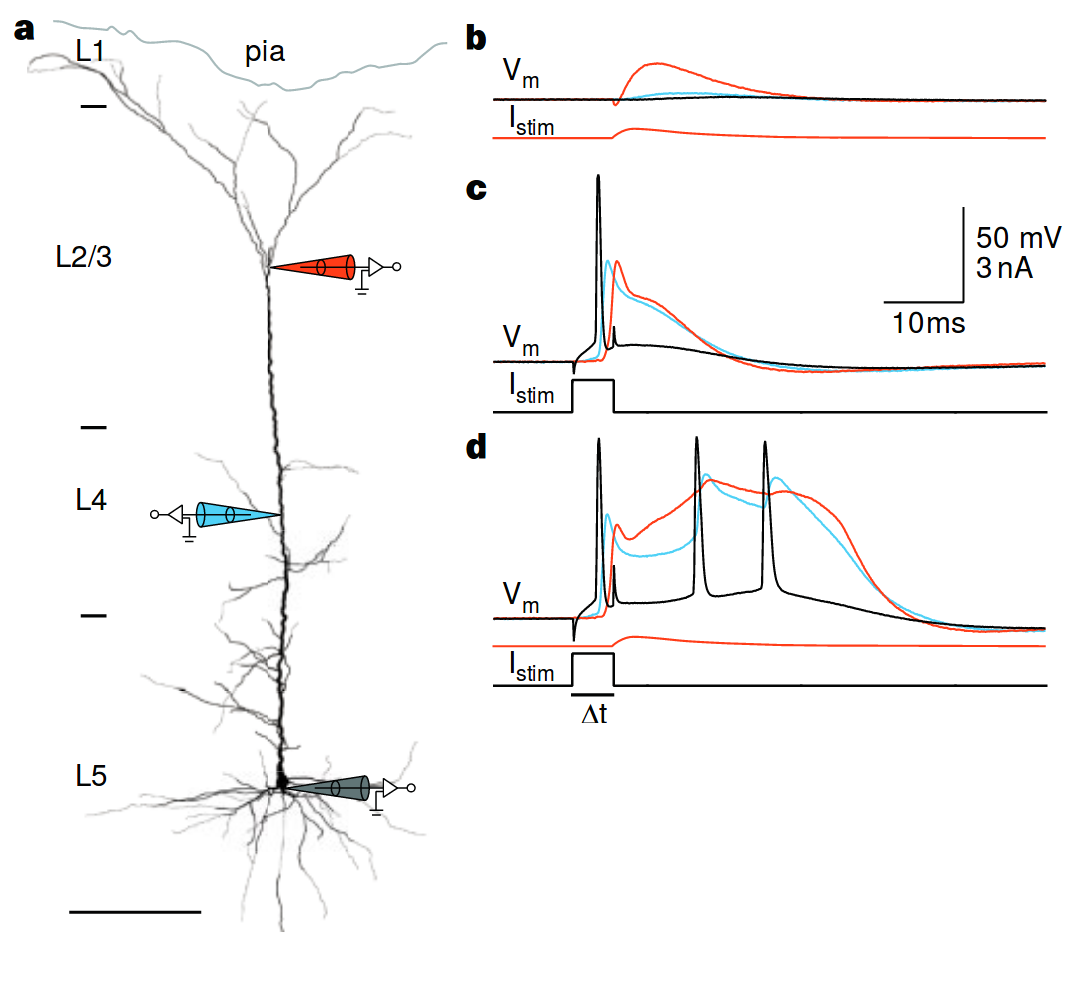
\includegraphics[width=0.5\columnwidth]{bac.png} 
\caption[BAC Firing]{From Larkum 1999. \textbf{a}, schematic of pyramidal neuron with indication of injection/recording sites. The gray pipette is positioned at the soma. \textbf{b}, EPSP-shaped injection at distal dendritic tuft, no injection at the soma. The signal is very weak whent it arrives at the soma and is not sufficient for any kind of AP. \textbf{c}, Injection at soma but not at the distal dendritic tuft. We see a sodium-AP but no BAC firing, since the threshold for a dendritic AP has not been reached. \textbf{d},  Injections at soma and distal dendritic tuft. We see dendritic spikes and a burst of APs at the soma.} % The text in the square bracket is the caption for the list of figures while the text in the curly brackets is the figure caption
\label{fig:bac} 
\end{figure}

Figure \ref{fig:bac} (from \cite{Larkum1999}) shows the effect of BAC firing. As shown in panels a and b, EPSPs coming in from the dendrites or an axonal action potential alone are not sufficient to bring about BAC firing, but a combination of the two is, as seen in panel c. We see that BAC firing results in a burst of spikes.

Since the dendritic tree of L5 pyramidal neurons extends into other layers of the cortex, this behavior opens up the possibility of BAC firing being a key machanism in linking together different aspects of a sensory experience \cite{Larkum1999}. This would mean that the dendritic activity of these neurons carries vital information about perception and perception-related behavior.

%------------------------------------------------

\section{The Experiment}
Building on the previously described findings, a perceptual experiment was conducted by Naoya Takahashi (et al?), and the respective findings were published in \cite{Takahashi2016}. The data from this experiment constitute the basis for the work described in this report.

The setup is as follows: Adult mice were put on a water restriction and had a metal bar attatched to their C2 whisker. Afterwards, the metal bar was deflected with varying intensties (seven different ones including a zero-stimulus for each mouse, calibrated such that the middle stimulus was as close as possible the the detection threshold of the mouse) with the help of a magnetic coil placed underneath the mouse. The mouse's task was to detect the deflection and signal this by licking a sensor. On correct detection the mouse was given a water reward \cite{Takahashi2016}.

\begin{figure}[tb]
\centering 
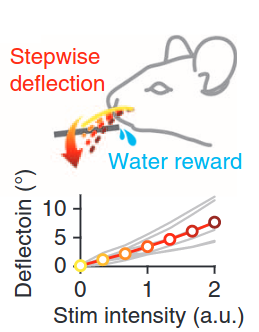
\includegraphics[width=0.5\columnwidth]{mouse.png} 
\caption[BAC Firing]{From Takahashi 2016. One example of the different stimuli and the respective deflection angels of the whiskers. For this particular animal, the maximum stimulus was two.} % The text in the square bracket is the caption for the list of figures while the text in the curly brackets is the figure caption
\label{fig:mouse} 
\end{figure}

Figure \ref{fig:mouse} shows one example of the stimulus array for one animal.

While the mice, which all expressed a flourescent proteine that bound to Ca$^{2+}$ performed the task, two-photon microscopy was performed, imaging a 175 by 175 $\mu$m plane with 98.1 $\pm$ 17.8 apical dendrites (correct numbers!), capturing the Ca$^{2+}$ activity over time (3 seconds, one prestimulus and two post).
\begin{figure}[tb]
\centering 
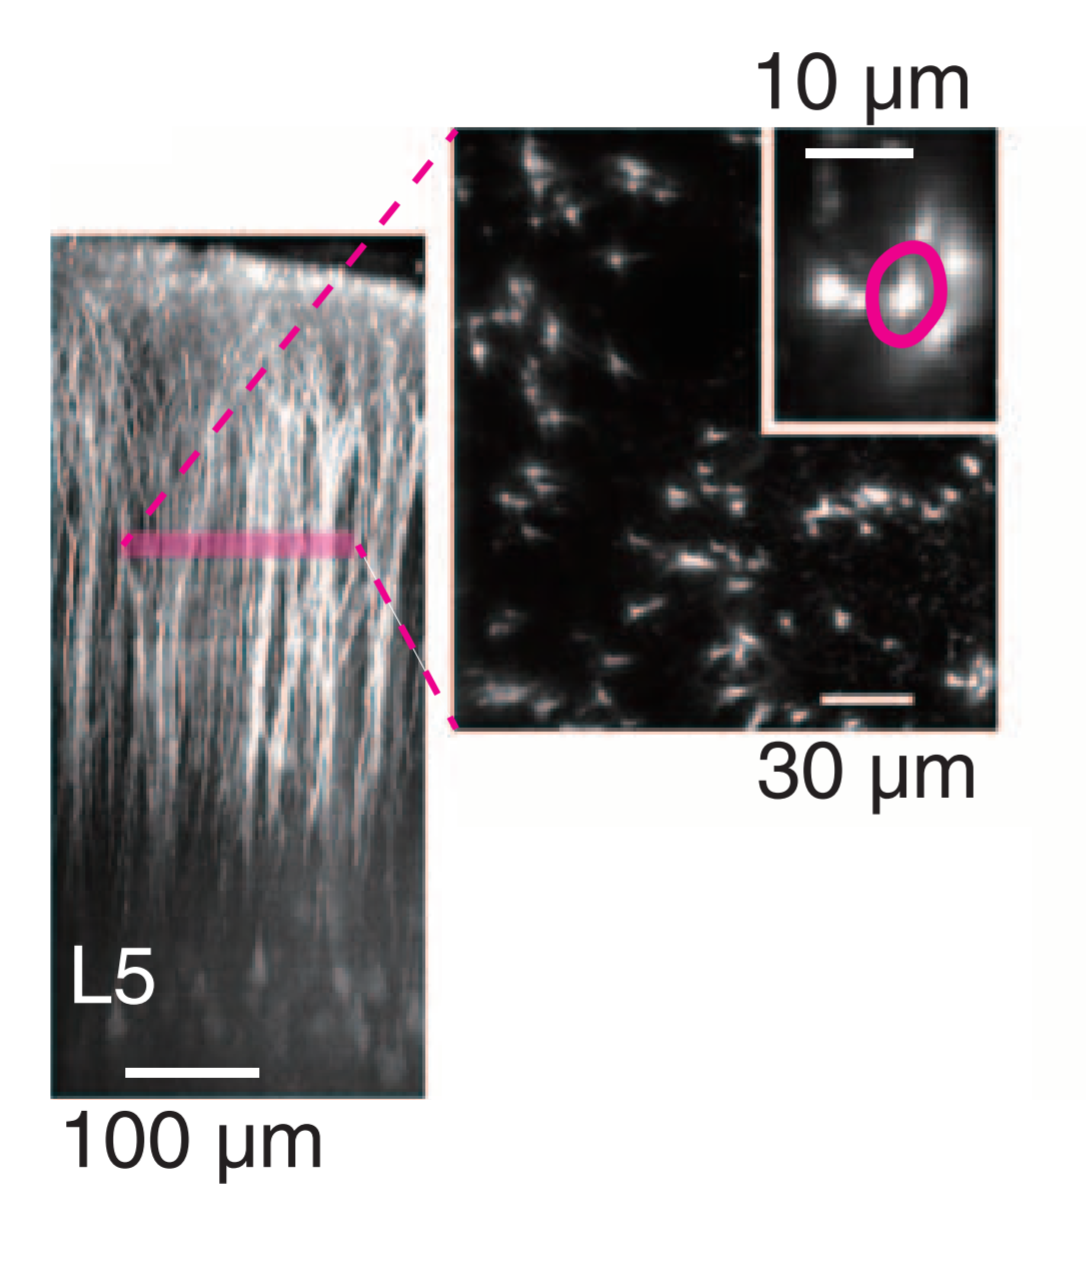
\includegraphics[width=0.5\columnwidth]{roi.png} 
\caption[BAC Firing]{From Takahashi 2016. \textbf{left}, crossection of L5 pyramidal neurons with their dendritic trees and the location of the imaging plane. \textbf{right}, the imaging plane. The white dots all represent a dendrtie.} % The text in the square bracket is the caption for the list of figures while the text in the curly brackets is the figure caption
\label{fig:roi} 
\end{figure}
In figure \ref{fig:roi} we see how the field of view looks like and where in the cortex the recording was made.

The training sessions in which the association between stimulus and reward was established were not included in the data used for analysis.

Here go psychometric curve etc.

\section{Original Results}
In this section we briefly go over some of the results obtained from the experiment described above.                                                                                                                                                                                 
As mentioned before, univariate analysis was performed in \cite{Takahashi2016} for each individual dendrite in order to find out how much its activity correlated with the stimulus. 
\subsection{Math}

\lipsum[4] % Dummy text

\begin{equation}
\cos^3 \theta =\frac{1}{4}\cos\theta+\frac{3}{4}\cos 3\theta
\label{eq:refname2}
\end{equation}

\lipsum[5] % Dummy text

\begin{definition}[Gauss] 
To a mathematician it is obvious that
$\int_{-\infty}^{+\infty}
e^{-x^2}\,dx=\sqrt{\pi}$. 
\end{definition} 

\begin{theorem}[Pythagoras]
The square of the hypotenuse (the side opposite the right angle) is equal to the sum of the squares of the other two sides.
\end{theorem}

\begin{proof} 
We have that $\log(1)^2 = 2\log(1)$.
But we also have that $\log(-1)^2=\log(1)=0$.
Then $2\log(-1)=0$, from which the proof.
\end{proof}

%----------------------------------------------------------------------------------------
%	RESULTS AND DISCUSSION
%----------------------------------------------------------------------------------------

\section{Results and Discussion}

Reference to Figure~\vref{fig:gallery}. % The \vref command specifies the location of the reference

\begin{figure}[tb]
\centering 
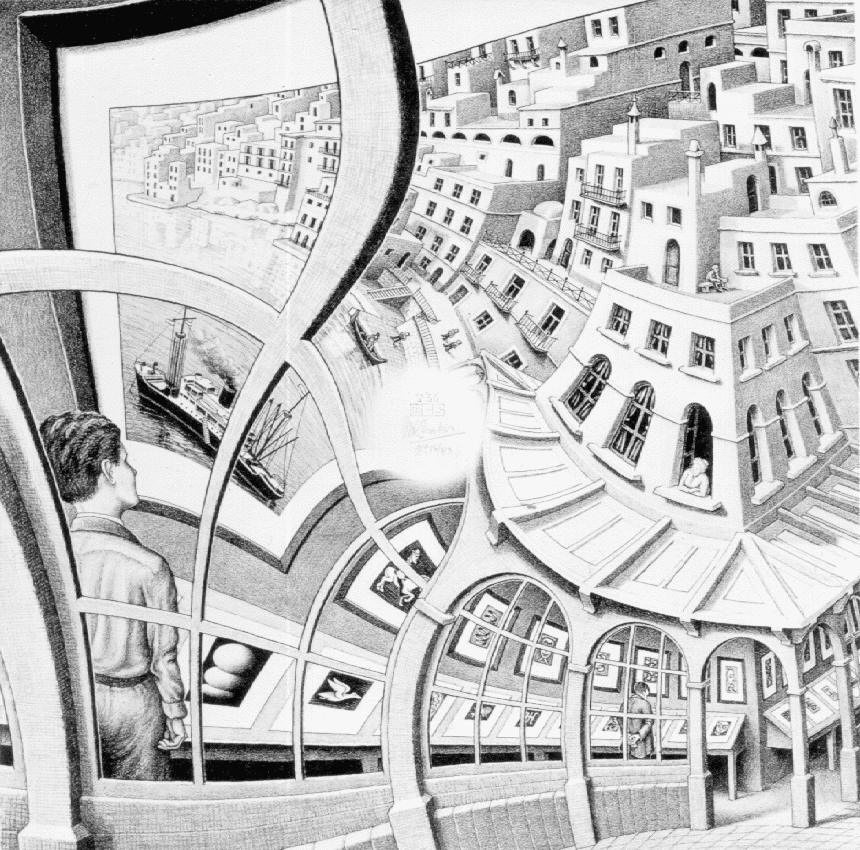
\includegraphics[width=0.5\columnwidth]{GalleriaStampe} 
\caption[An example of a floating figure]{An example of a floating figure (a reproduction from the \emph{Gallery of prints}, M.~Escher,\index{Escher, M.~C.} from \url{http://www.mcescher.com/}).} % The text in the square bracket is the caption for the list of figures while the text in the curly brackets is the figure caption
\label{fig:gallery} 
\end{figure}

\lipsum[10] % Dummy text

%------------------------------------------------

\subsection{Subsection}
\lipsum[11] % Dummy text

\subsubsection{Subsubsection}

\lipsum[12] % Dummy text

\begin{description}
\item[Word] Definition
\item[Concept] Explanation
\item[Idea] Text
\end{description}

\lipsum[12] % Dummy text

\begin{itemize}[noitemsep] % [noitemsep] removes whitespace between the items for a compact look
\item First item in a list
\item Second item in a list
\item Third item in a list
\end{itemize}

\subsubsection{Table}

\lipsum[13] % Dummy text

\begin{table}[hbt]
\caption{Table of Grades}
\centering
\begin{tabular}{llr}
\toprule
\multicolumn{2}{c}{Name} \\
\cmidrule(r){1-2}
First name & Last Name & Grade \\
\midrule
John & Doe & $7.5$ \\
Richard & Miles & $2$ \\
\bottomrule
\end{tabular}
\label{tab:label}
\end{table}

Reference to Table~\vref{tab:label}. % The \vref command specifies the location of the reference

%------------------------------------------------

\subsection{Figure Composed of Subfigures}

Reference the figure composed of multiple subfigures as Figure~\vref{fig:esempio}. Reference one of the subfigures as Figure~\vref{fig:ipsum}. % The \vref command specifies the location of the reference

\lipsum[15-18] % Dummy text

\begin{figure}[tb]
\centering
\subfloat[A city market.]{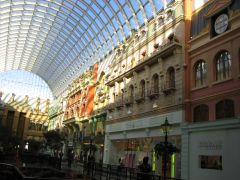
\includegraphics[width=.45\columnwidth]{Lorem}} \quad
\subfloat[Forest landscape.]{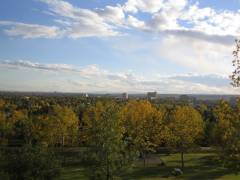
\includegraphics[width=.45\columnwidth]{Ipsum}\label{fig:ipsum}} \\
\subfloat[Mountain landscape.]{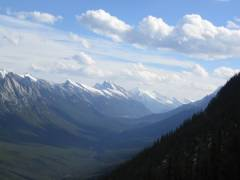
\includegraphics[width=.45\columnwidth]{Dolor}} \quad
\subfloat[A tile decoration.]{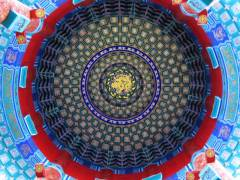
\includegraphics[width=.45\columnwidth]{Sit}}
\caption[A number of pictures.]{A number of pictures with no common theme.} % The text in the square bracket is the caption for the list of figures while the text in the curly brackets is the figure caption
\label{fig:esempio}
\end{figure}

%----------------------------------------------------------------------------------------
%	BIBLIOGRAPHY
%----------------------------------------------------------------------------------------

\renewcommand{\refname}{\spacedlowsmallcaps{References}} % For modifying the bibliography heading

\bibliographystyle{unsrt}

\bibliography{sample.bib} % The file containing the bibliography

%----------------------------------------------------------------------------------------

\end{document}